\section{Thomsonov problem}

Želimo poiskati minimum elektrostatične energija pri razporeditvi $N$ enakih nabojev po krogli 
\begin{equation}
    E = \sum_{i, j>i}^N \frac{1}{\abs{\Vec{r}_i - \Vec{r}_j}} =  \text{MIN}
\end{equation}
kjer so $\Vec{r}$ krajevni vektorji nabojev. Primer obravnavamo brezdimenzijsko, za iskanje minimuma uporabimo numerično minimizacijo v več dimenzijah, v našem primeru metodo Neldel-Mead oz. \textit{ameba}, metodo Powell, metodo konjugiranih gradientov (CG) in metodo Broyden–Fletcher–Goldfarb–Shanno (BFGS). 

Na sliki \ref{fig:porazdelitev} je prikazana porazdelitev nabojev za nekaj primerov, v primeru velikega števila nabojev je prikaz nepregleden, zato ni prikazan. Dalje slika \ref{fig:energija} prikazuje, kako se spreminja skupna energija sistema in energija na en naboj. Pričakovano je, da skupna energija narašča eksponentno, zanimivo pa je, da energija na delec narašča linearno. V tem primeru ni zaznati večjih razlik pri izračunu z različnimi metodami.
\begin{figure}[ht!]
\begin{centering}
    \begin{subfigure}[b]{.3\textwidth}
        \centering 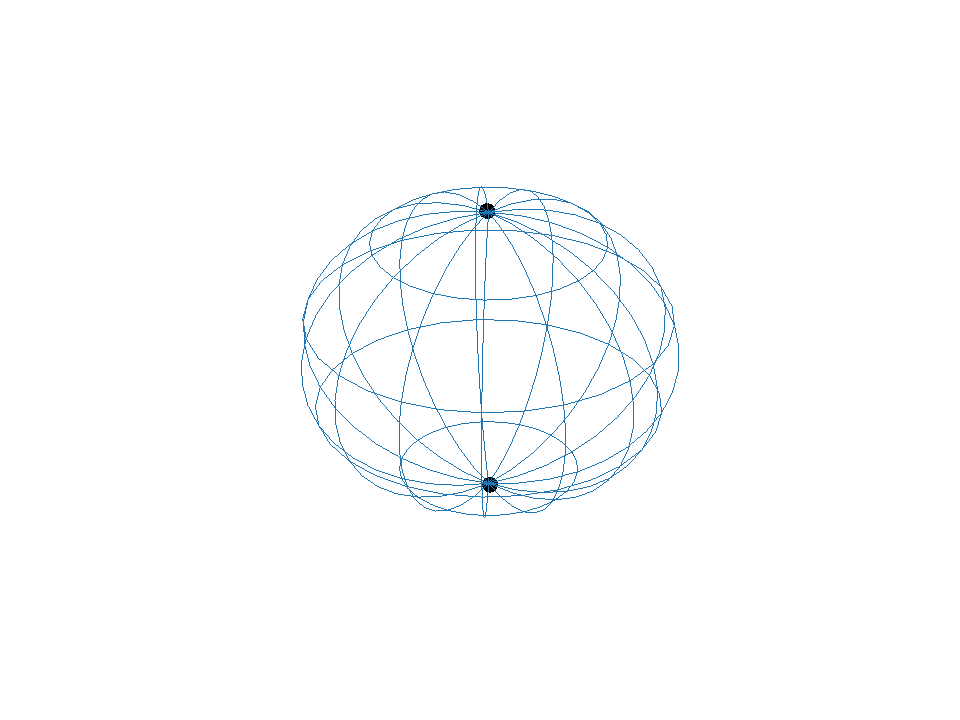
\includegraphics[scale=0.4]{3.nal slike/porazdelitev_n_2.pdf}
    \end{subfigure}
    \quad
    \begin{subfigure}[b]{.3\textwidth}
        \centering 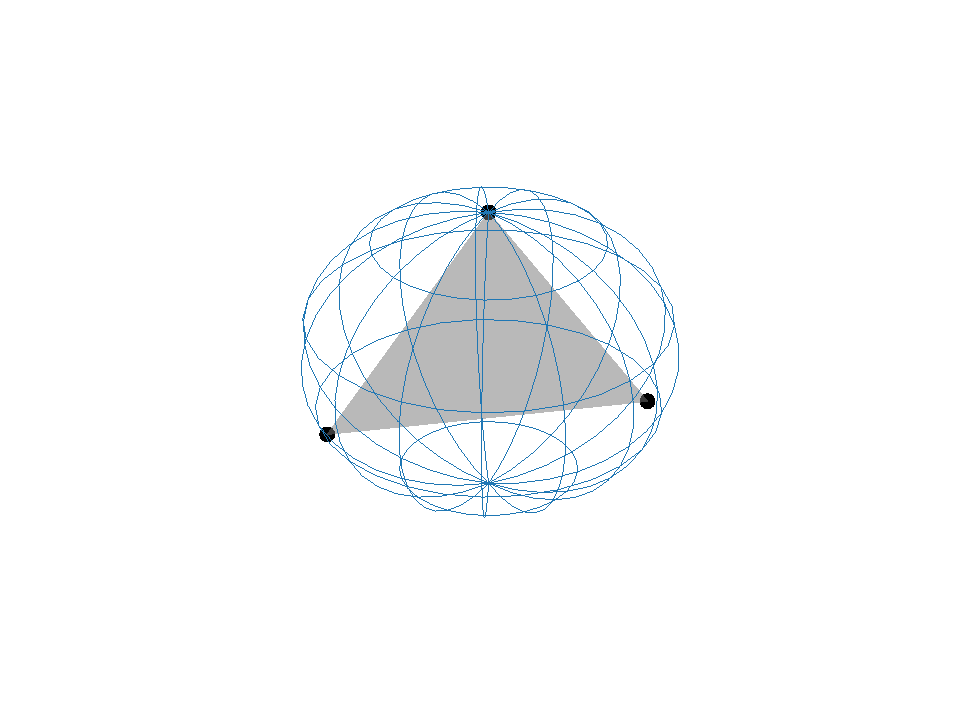
\includegraphics[scale=0.4]{3.nal slike/porazdelitev_n_3.pdf}
    \end{subfigure}
    \quad
    \begin{subfigure}[b]{.3\textwidth}
        \centering 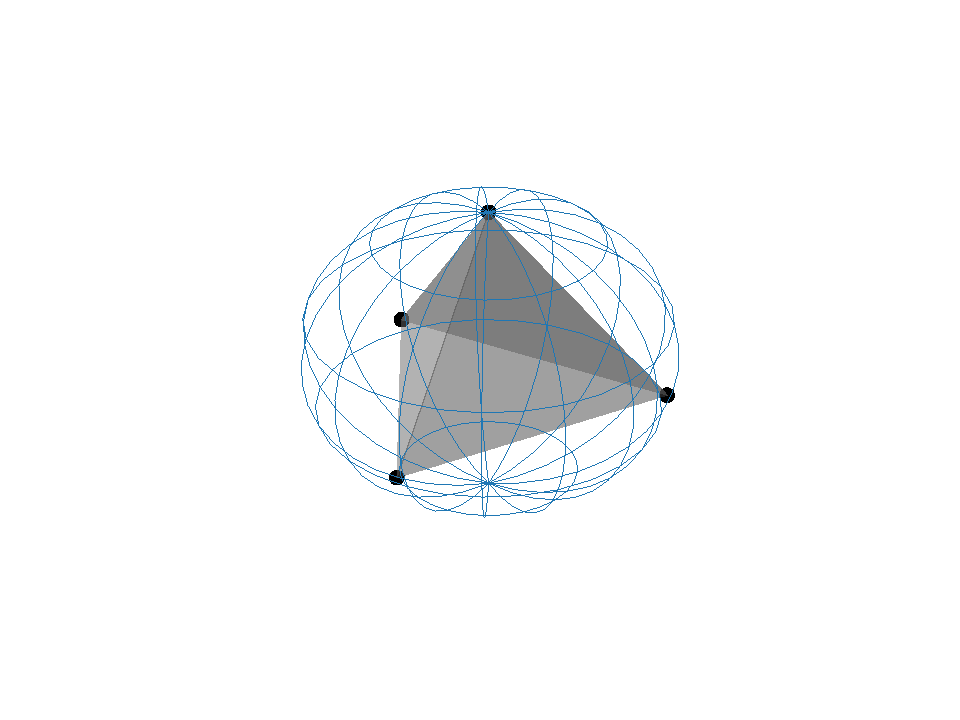
\includegraphics[scale=0.4]{3.nal slike/porazdelitev_n_4.pdf}
    \end{subfigure}
    \quad
    \begin{subfigure}[b]{.3\textwidth}
        \centering 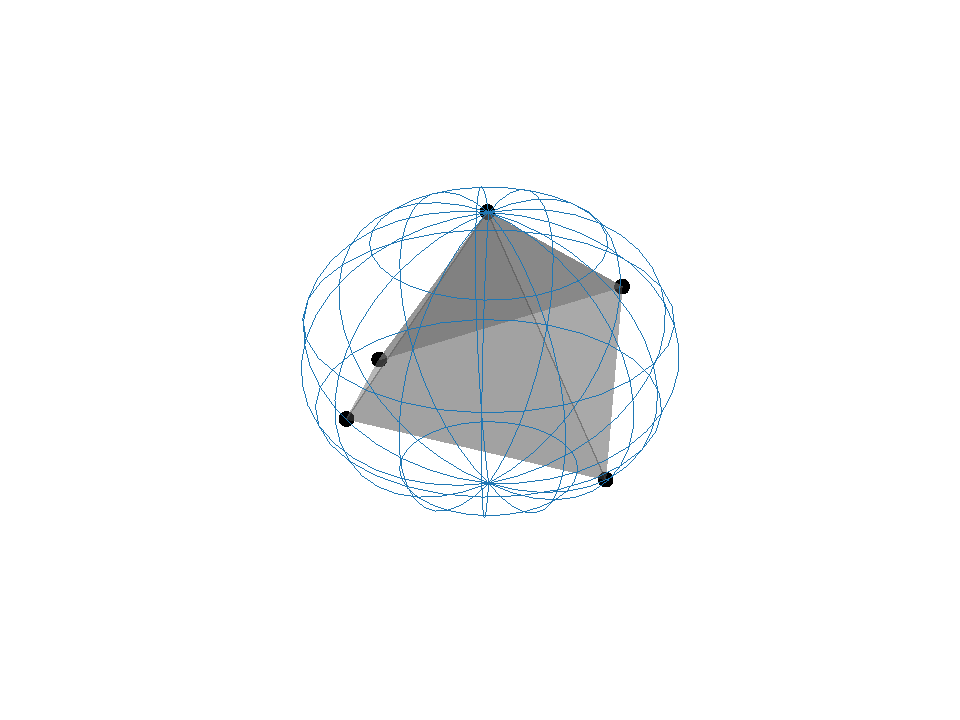
\includegraphics[scale=0.4]{3.nal slike/porazdelitev_n_5.pdf}
    \end{subfigure}
    \quad
    \begin{subfigure}[b]{.3\textwidth}
        \centering 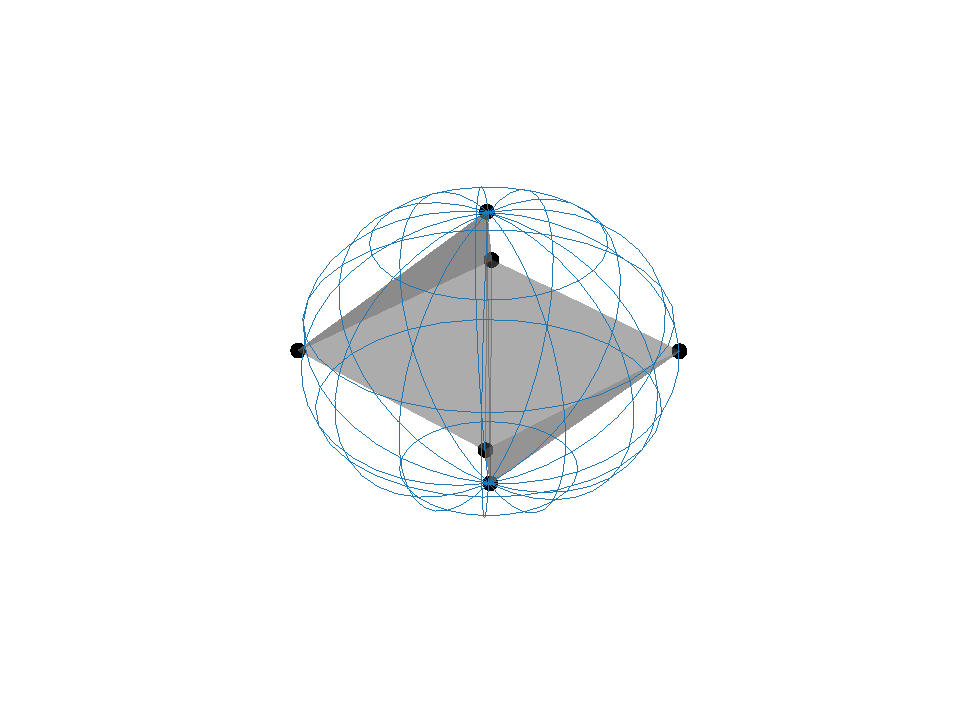
\includegraphics[scale=0.4]{3.nal slike/porazdelitev_n_6.pdf}
    \end{subfigure}
    \quad
    \begin{subfigure}[b]{.3\textwidth}
        \centering 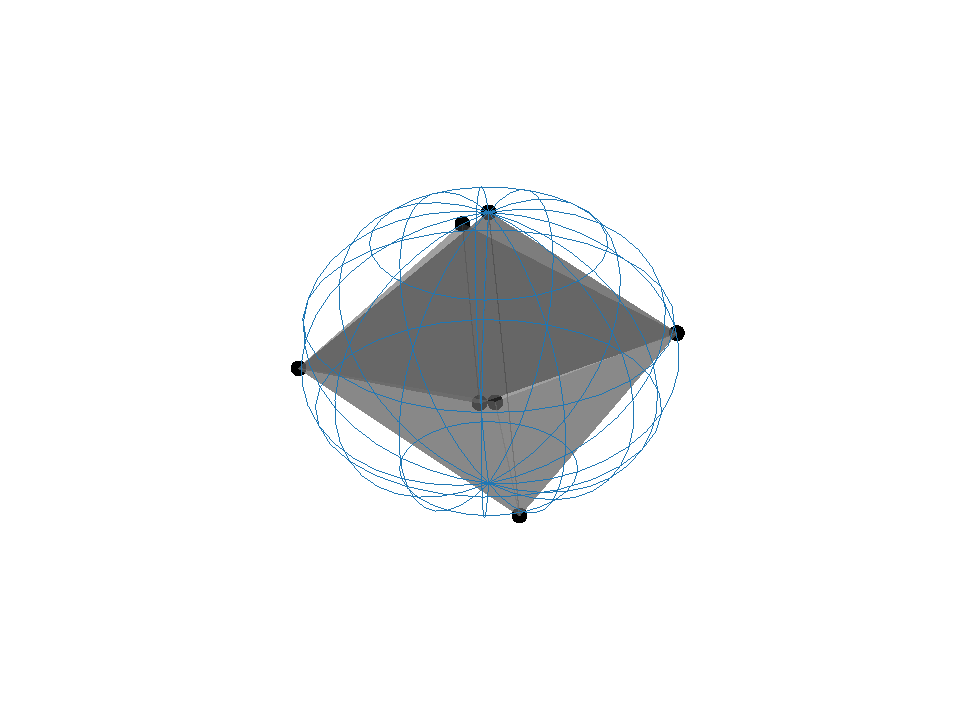
\includegraphics[scale=0.4]{3.nal slike/porazdelitev_n_7.pdf}
    \end{subfigure}
    \quad
    \caption{Porazdelitev nabojev po krogli}
    \label{fig:porazdelitev}
\end{centering}
\end{figure}
\begin{figure}[ht!]
    \centering
    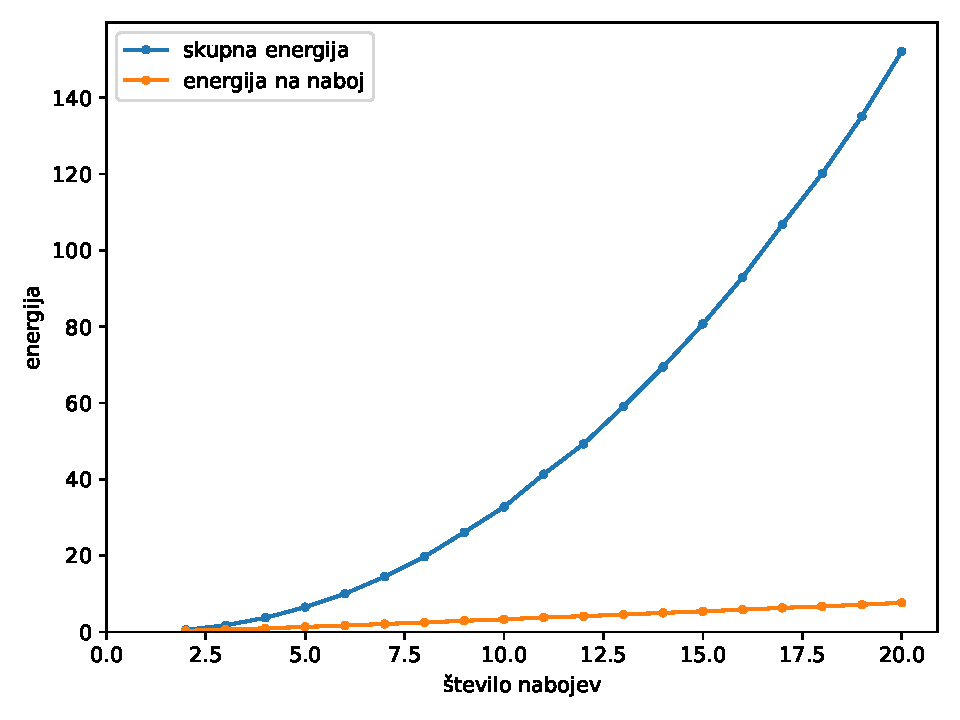
\includegraphics[width=0.8\textwidth]{3.nal slike/skupna_E_in_E_na_delec.pdf}
    \caption{Energija na naboj in skupna energija}
    \label{fig:energija}
\end{figure}
\newpage
Primerjave metod so vidne na sliki \ref{fig:iteracije}, kjer je zanimivo, da število iteracij amebe narašča skoraj linearno, metoda konjugiranih gradientov pa zelo niha. Kot najbolj učinkoviti se izkažeta metodi Powell in BFGS. Za časovno najbolj učinkovito se izkaže metoda Powell, kot je prikazano v tabeli \ref{tab:čas}. Pri manjših številih nabojev je računski čas dokaj majhen za vse metode, z večanjem pa lahko stvari hitro zapletemo...
\begin{figure}[ht!]
    \centering
    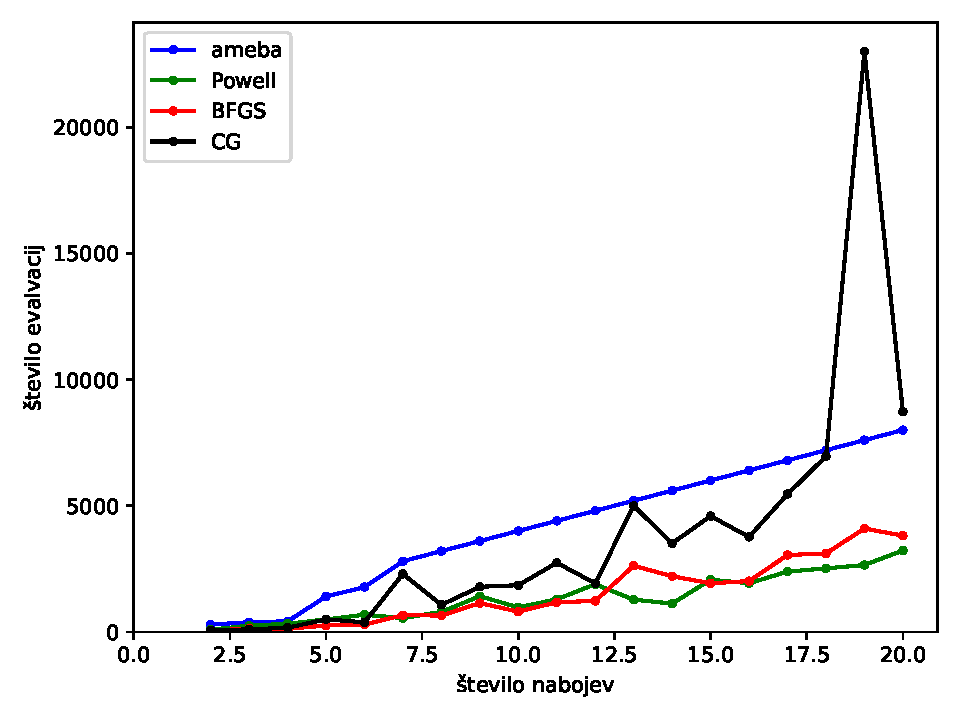
\includegraphics[width=0.8\textwidth]{3.nal slike/št_iteracij.pdf}
    \caption{Število iteracij za različne metode}
    \label{fig:iteracije}
\end{figure}
\begin{table}[ht!]
    \centering
    \begin{tabular}{c|c|c|c|c}
        število nabojev & ameba & Powell & BFGS & CG \\
        \hline
        22 & 14,0 s & 6,2 s & 6,1 s & 14,8 s \\
        25 & 20,9 s & 6,4 s & 20,3 s & 98,4 s \\
    \end{tabular}
    \caption{Časovno trajanje numerične minimizacije}
    \label{tab:čas}
\end{table}

\section{Vožnja mimo semaforja}

Obravnavamo isti problem iz 1. naloge, ki ga tokrat rešujemo numerično, zato iskani minimum pospeška prepišemo v diskretno obliko
\begin{equation}
    F = 0,5 \, \left(\frac{v_0}{\Delta t}\right)^2 + \sum_{i=1}^{N-1} \left(\frac{v_i - v_{i-1}}{\Delta t}\right)^2 + 0,5 \, \left(\frac{v_N}{\Delta t}\right)^2 = \text{MIN}
\end{equation}
Vez za pogoj prevožene razdalje $\int_0^{t_0} v(t) \, dt = L$ implementiramo diskretno v obliki
\begin{equation}
    0,5 \, v_0 + \sum_{i=1}^{N-1} v_i + 0,5 \, v_N \leq L
\end{equation}
tako, da se minimizirajoča funkcija sedaj glasi 
\begin{equation}
    F = 0,5 \, \left(\frac{v_0}{\Delta t}\right)^2 + \sum_{i=1}^{N-1} \left(\frac{v_i - v_{i-1}}{\Delta t}\right)^2 + 0,5 \, \left(\frac{v_N}{\Delta t}\right)^2 + \exp\left[ \kappa \left(0,5 \, v_0 + \sum_{i=1}^{N-1} v_i + 0,5 \, v_N - \frac{L}{\Delta t}\right)\right]
\end{equation}


Na sliki \ref{fig:primerjava_hitr} so prikazani izračuni za $t_0 = 1$, $L = 1$, $\kappa = 1$ in različne $v_0$, pri numerične izračunu je uporabljenih $N = 20$ računskih točk. Opazna so odstopanja od analitike vendar je potek hitrosti dokaj skladen. Pri $v_0=0$ je mejni primer, saj je končna hitrost enaka 0, in pri povečevanju $v_0$ prihaja do negativne hitrosti oz. vožnje nazaj. Na sliki \ref{fig:primerjava_pot} je to opazno še bolj opazno, saj v želji po minimizaciji vezi, ki implementira pogoj $\int_0^{t_0} v(t) \, dt = L$, program ustvarja rešitve, ki pa niso uporabne.
\begin{figure}[H]
    \centering
    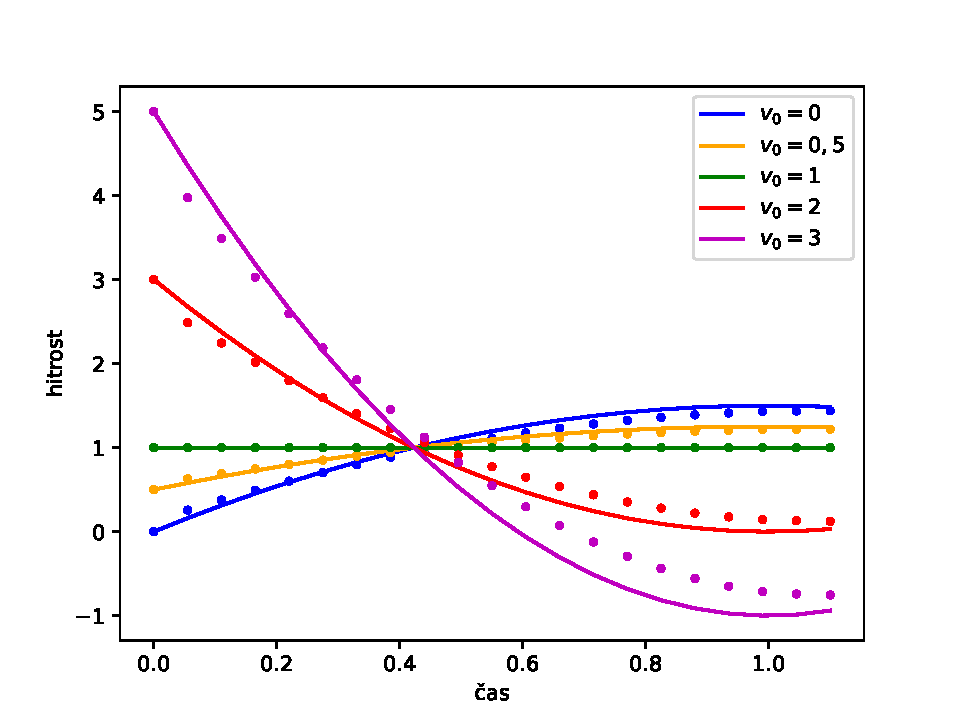
\includegraphics[width=0.8\textwidth]{3.nal slike/primerjava_z analitično.pdf}
    \caption{Primerjava med analitičnimi (črte) in numeričnimi rešitvami (točke) za različne začetne hitrosti}
    \label{fig:primerjava_hitr}
\end{figure}
\begin{figure}[ht!]
    \centering
    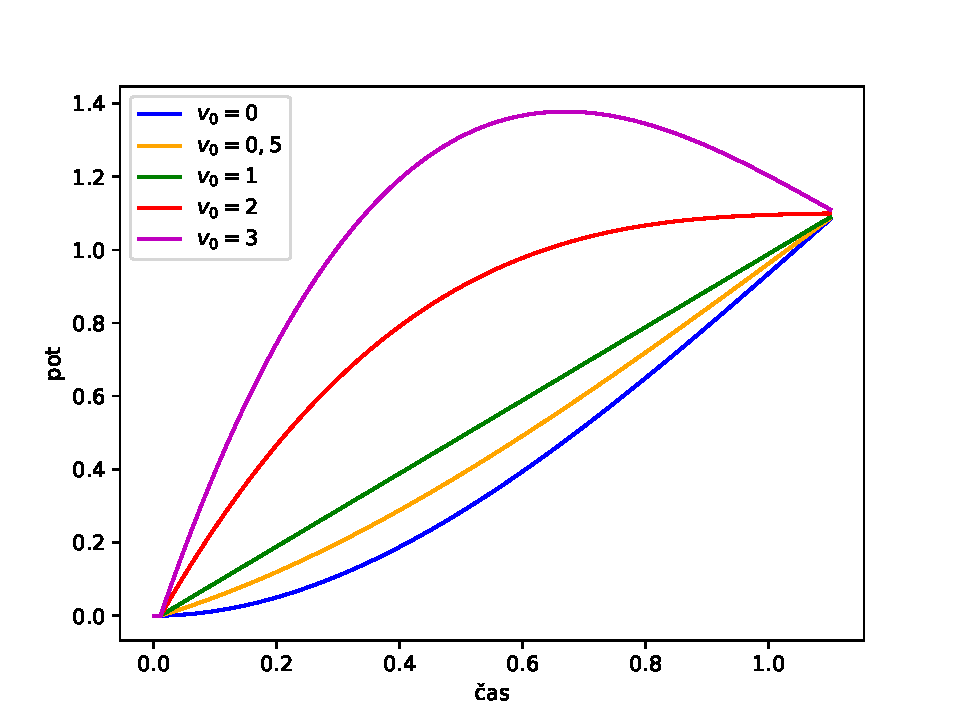
\includegraphics[width=0.8\textwidth]{3.nal slike/pot.pdf}
    \caption{Potek poti za različne začetne hitrosti}
    \label{fig:primerjava_pot}
\end{figure}
\newpage
Pri zviševanju števila računskih točk, torej manjšanju časovne diskretizacije, je moč opaziti približevanje analitični rešitvi, vendar pri številu točk nad 100 pride do primera, ki zgleda kot zlomljen graf, čemur vzrok ni znan.
\begin{figure}[!ht]
    \centering
    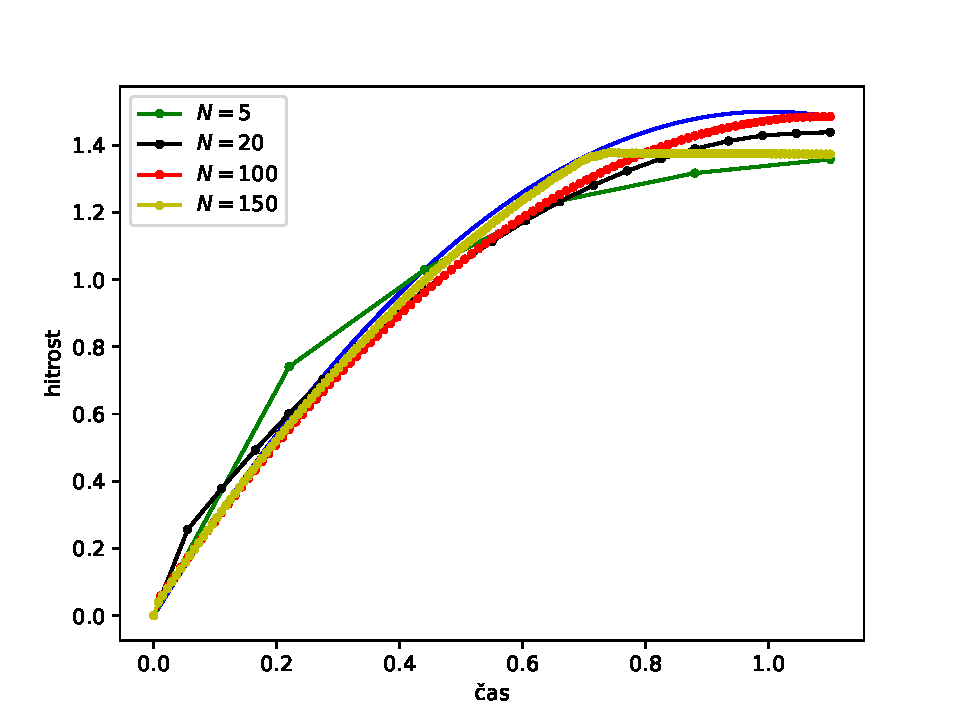
\includegraphics[width=0.8\textwidth]{3.nal slike/vpliv_N.pdf}
    \caption{Vpliv števila točk na rezultat}
    \label{fig:vpliv_N}
\end{figure}
\newpage
Na sliki \ref{fig:kapa} sem večal pomembnost vezi, in tako ugotovil, da le to teži k vedno bolj konstantni hitrosti.
\begin{figure}[ht!]
    \centering
    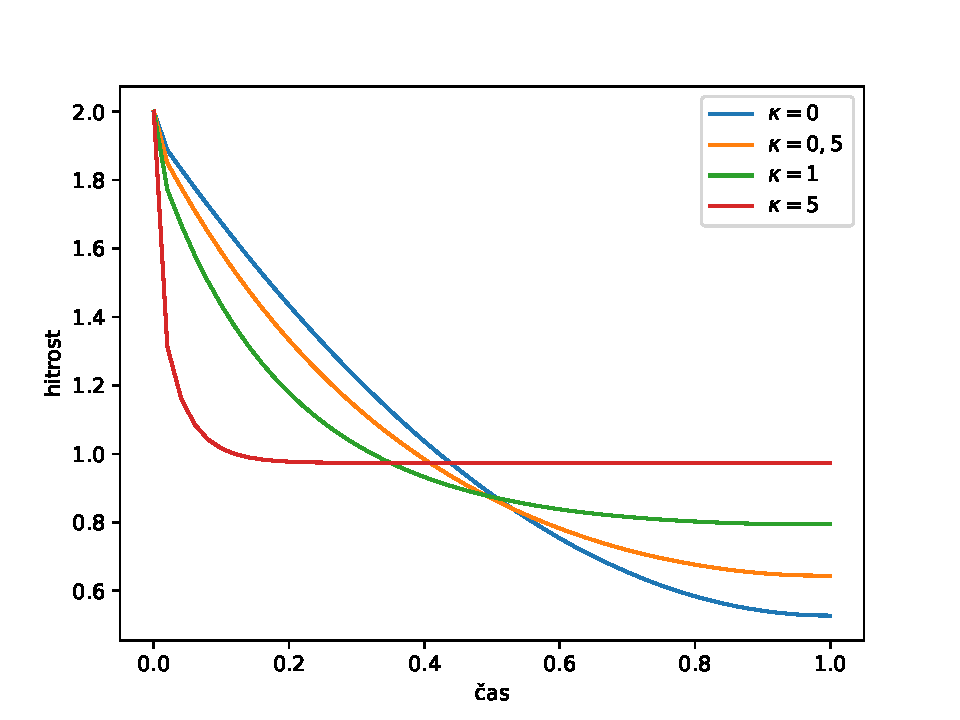
\includegraphics[width=0.8\textwidth]{3.nal slike/vpliv_kapa.pdf}
    \caption{Vpliv parametra $\kappa$}
    \label{fig:kapa}
\end{figure}